% SSM: three equivalent evaluation schedules — TikZ source. Compiles to a tight
% standalone PDF (pdflatex figures/ssm-three-faces.tex), which
% `book-scaffold build-figures` converts to public/figures/ssm-three-faces.svg
% (PDF -> SVG via pdftocairo).
%
% One linear recurrence h_t = Abar h_{t-1} + Bbar u_t, y_t = C h_t (n=4 steps),
% evaluated three ways: sequential recurrence (decode, O(1) state per token),
% a fixed convolution kernel kappa_j = C Abar^j Bbar applied in one FFT pass
% (whole input known up front), and a depth-ceil(log2 n) associative-scan tree
% over affine pairs (a_t,b_t) (train, parallel). Same map, three schedules.
\documentclass[tikz,border=3pt]{standalone}
\usepackage{amsmath}
\usepackage{amssymb}
\usepackage{tikz}
\usetikzlibrary{positioning,arrows.meta,calc,fit}
\begin{document}
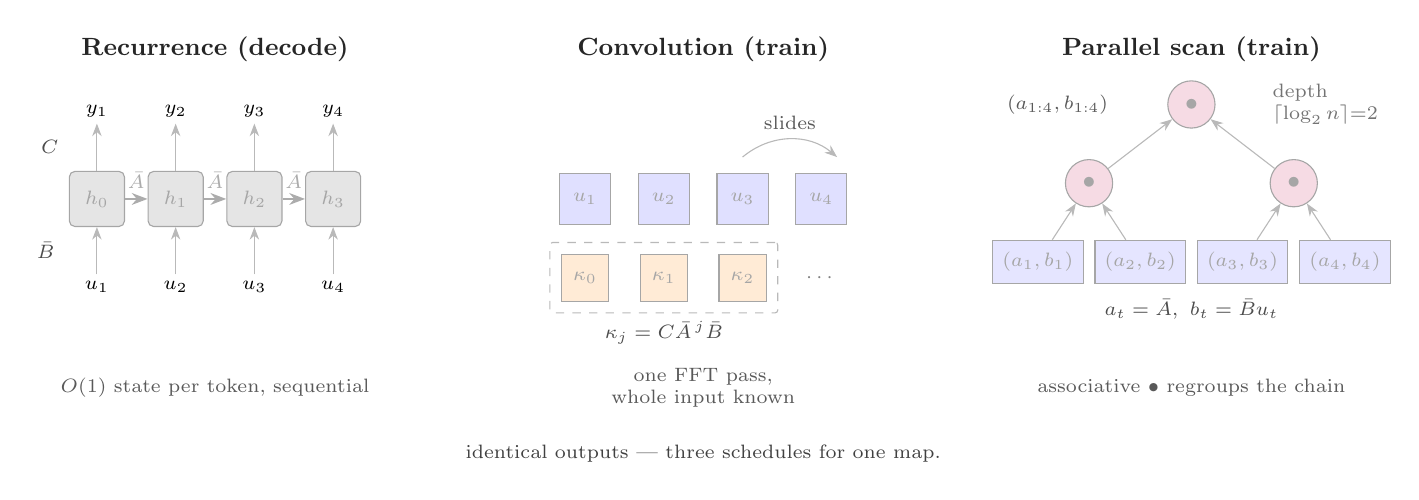
\begin{tikzpicture}[
    font=\small,
    state/.style={draw, gray!70, rounded corners=2pt, fill=black!10,
                  minimum size=7mm, inner sep=1pt, font=\scriptsize},
    seq/.style={->, >={Stealth[length=2.0mm]}, gray!65, thick},
    io/.style={->, >={Stealth[length=1.6mm]}, gray!55},
    intok/.style={draw, gray!70, fill=blue!12, minimum size=6.5mm, inner sep=1pt,
                  font=\scriptsize},
    kern/.style={draw, gray!70, fill=orange!16, minimum size=6mm, inner sep=1pt,
                 font=\scriptsize},
    leaf/.style={draw, gray!70, fill=blue!10, minimum width=11.5mm,
                 minimum height=5.5mm, inner sep=1pt, font=\scriptsize},
    comb/.style={draw, gray!70, circle, fill=purple!14, minimum size=6mm,
                 inner sep=0pt, font=\small},
    ttl/.style={font=\small\bfseries, text=black!85},
    note/.style={font=\scriptsize, text=black!65, align=center},
  ]

  % ============================== Panel 1 =================================
  % Recurrence (decode): h_t = Abar h_{t-1} + Bbar u_t, y_t = C h_t.
  \begin{scope}
    \node[state] (h0) at (-15mm,0) {$h_0$};
    \node[state] (h1) at (-5mm,0)  {$h_1$};
    \node[state] (h2) at (5mm,0)   {$h_2$};
    \node[state] (h3) at (15mm,0)  {$h_3$};

    \draw[seq] (h0) -- (h1) node[midway, above, font=\scriptsize] {$\bar A$};
    \draw[seq] (h1) -- (h2) node[midway, above, font=\scriptsize] {$\bar A$};
    \draw[seq] (h2) -- (h3) node[midway, above, font=\scriptsize] {$\bar A$};

    \foreach \n/\t in {h0/1, h1/2, h2/3, h3/4} {
      \draw[io] ($(\n.south)+(0,-6mm)$) -- (\n.south);
      \node[font=\scriptsize] at ($(\n.south)+(0,-7.6mm)$) {$u_\t$};
      \draw[io] (\n.north) -- ($(\n.north)+(0,6mm)$);
      \node[font=\scriptsize] at ($(\n.north)+(0,7.6mm)$) {$y_\t$};
    }
    \node[font=\scriptsize, text=black!70] at ($(h0.south)+(-6.5mm,-3mm)$) {$\bar B$};
    \node[font=\scriptsize, text=black!70] at ($(h0.north)+(-6mm,3mm)$) {$C$};

    \node[ttl] at (0,19mm) {Recurrence (decode)};
    \node[note, text width=40mm] at (0,-24mm) {$O(1)$ state per token, sequential};
  \end{scope}

  % ============================== Panel 2 =================================
  % Convolution (train): y = kappa * u, kappa_j = C Abar^j Bbar, one kernel.
  \begin{scope}[xshift=62mm]
    \node[intok] (u1) at (-15mm,0) {$u_1$};
    \node[intok] (u2) at (-5mm,0)  {$u_2$};
    \node[intok] (u3) at (5mm,0)   {$u_3$};
    \node[intok] (u4) at (15mm,0)  {$u_4$};

    \node[kern] (k0) at (-15mm,-10mm) {$\kappa_0$};
    \node[kern] (k1) at (-5mm,-10mm)  {$\kappa_1$};
    \node[kern] (k2) at (5mm,-10mm)   {$\kappa_2$};
    \node[font=\scriptsize, text=black!50] (kd) at (15mm,-10mm) {$\cdots$};

    \node[draw, gray!55, dashed, rounded corners=1pt, fit=(k0)(k1)(k2),
          inner sep=1.4mm] (kwin) {};

    \draw[io] ($(u3.north)+(0,2mm)$) to[bend left=40]
      node[midway, above, font=\scriptsize, text=black!65] {slides}
      ($(u4.north)+(2mm,2mm)$);

    \node[font=\scriptsize, text=black!70] at (-5mm,-17mm)
      {$\kappa_j = C\bar A^{\,j}\bar B$};

    \node[ttl] at (0,19mm) {Convolution (train)};
    \node[note, text width=40mm] at (0,-24mm) {one FFT pass, whole input known};
  \end{scope}

  % ============================== Panel 3 =================================
  % Parallel scan (train): associative combination of affine pairs (a_t,b_t).
  \begin{scope}[xshift=124mm]
    \node[leaf] (l1) at (-19.5mm,-8mm) {$(a_1,b_1)$};
    \node[leaf] (l2) at (-6.5mm,-8mm)  {$(a_2,b_2)$};
    \node[leaf] (l3) at (6.5mm,-8mm)   {$(a_3,b_3)$};
    \node[leaf] (l4) at (19.5mm,-8mm)  {$(a_4,b_4)$};

    \coordinate (mid12) at ($(l1)!0.5!(l2)$);
    \coordinate (mid34) at ($(l3)!0.5!(l4)$);
    \node[comb] (m1) at ($(mid12)+(0,10mm)$) {$\bullet$};
    \node[comb] (m2) at ($(mid34)+(0,10mm)$) {$\bullet$};
    \coordinate (midroot) at ($(m1)!0.5!(m2)$);
    \node[comb] (root) at ($(midroot)+(0,10mm)$) {$\bullet$};

    \draw[io] (l1) -- (m1);
    \draw[io] (l2) -- (m1);
    \draw[io] (l3) -- (m2);
    \draw[io] (l4) -- (m2);
    \draw[io] (m1) -- (root);
    \draw[io] (m2) -- (root);

    \node[font=\scriptsize, text=black!65, align=right] at ($(root)+(-17mm,0)$)
      {$(a_{1:4},b_{1:4})$};
    \node[font=\scriptsize, text=black!55, align=left] at ($(root)+(17mm,0)$)
      {depth\\$\lceil\log_2 n\rceil{=}2$};

    \node[font=\scriptsize, text=black!70] at (0,-14mm) {$a_t=\bar A,\ b_t=\bar B u_t$};

    \node[ttl] at (0,19mm) {Parallel scan (train)};
    \node[note, text width=40mm] at (0,-24mm) {associative $\bullet$ regroups the chain};
  \end{scope}

  % ============================== Footer ===================================
  \node[below, align=center, text width=15cm, font=\scriptsize, text=black!75]
    at (62mm,-30mm) {identical outputs --- three schedules for one map.};
\end{tikzpicture}
\end{document}
